\documentclass{standalone}
\usepackage{tikz}
\begin{document}

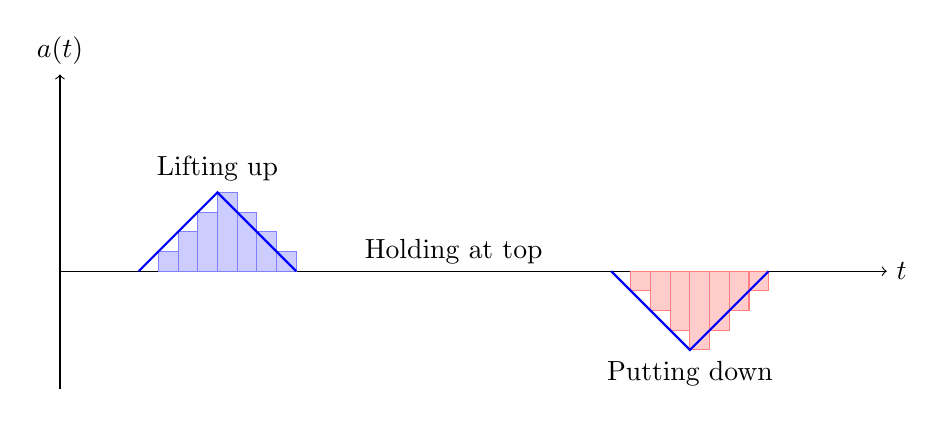
\begin{tikzpicture}[scale=1.0]

% Axes
\draw[->] (0,0) -- (10.5,0) node[right] {$t$};
\draw[->] (0,-1.5) -- (0,2.5) node[above] {$a(t)$};

% Rectangles under first triangle (1 to 3)
\foreach \x in {1,1.25,...,2.75} {
    % compute left and right x
    \pgfmathsetmacro{\xleft}{\x}
    \pgfmathsetmacro{\xright}{\x + 0.25}

    % compute height at left endpoint
    \pgfmathsetmacro{\yleft}{
        (\xleft>=1 && \xleft<=2) * (\xleft-1) +
        (\xleft>2 && \xleft<=3) * (-\xleft+3)
    }

    % only draw if height > 0
    \ifdim \yleft pt > 0pt
        \draw[fill=blue!20, draw=blue!50]
            (\xleft, 0) rectangle (\xright, \yleft);
    \fi
}

% Rectangles under second triangle (7 to 9)
\foreach \x in {7,7.25,...,8.75} {
    \pgfmathsetmacro{\xleft}{\x}
    \pgfmathsetmacro{\xright}{\x + 0.25}

    % compute height at left endpoint
    \pgfmathsetmacro{\yleft}{
        (\xleft>=7 && \xleft<8) * (-\xleft+7) +
        (\xleft>=8 && \xleft<=9) * (\xleft-9)
    }

    % only draw if height < 0
    \ifdim \yleft pt < 0pt
        \draw[fill=red!20, draw=red!50]
            (\xleft, 0) rectangle (\xright, \yleft);
    \fi
}

% Draw the piecewise function

% First triangle (1 to 3)
\draw[thick, blue]
    (1,0) -- (2,1) -- (3,0);

% Second triangle (7 to 9)
\draw[thick, blue]
    (7,0) -- (8,-1) -- (9,0);


% Labels
\node at (2, 1.3) {Lifting up};
\node at (8, -1.3) {Putting down};
\node at (5, 0.25) {Holding at top};

\end{tikzpicture}



\end{document}

